\cotefile{9}
\scanpage{2}
Dualité des modules de Dieudonné de \unsure{groupes|gpes} de B.T. \unsure{duels|duals} l'un de l'autre \unsure{\ldots---|\ldots|\ldots..}

Le module de Dieudonné réduit
\[
M\otimes_{W} k
\]
% archive sheet number: 1

\scanpage{3}
$k$ corps de car $p\unsure{\mathord{-}|>}0$

$G$ gpe $p$-divisible, $G^{*}$ dual

$g=\dim G,\quad g^{*}=\dim G^{*}$

$\widetilde G$ \unsure{gpe|groupe} enveloppant
\[
0\longrightarrow\underline{\mathbb V}(t_{G^{*}})\longrightarrow\widetilde G\longrightarrow G\longrightarrow0
\]

\diagram{\scriptsize\begin{tikzcd}[ampersand replacement=\&,column sep=.38em,row sep=.52em,cells={nodes={inner sep=1pt}}]
\&\&\&\&\&\text{duales}\arrow[ddd,dash]\&\&\&\&\&\\
0\arrow[r]\&t_G^\vee\arrow[r]\&H(G)\arrow[r]\arrow[dd,shift right,"{H(V)=V_0}"']\&t_{G^*}\arrow[r]\&0\&\&0\arrow[r]\&t_{G^*}^\vee\arrow[r]\&t_{\widetilde G}\arrow[r]\arrow[dd,shift right,"{V_0}"']\&t_G\arrow[r]\&0\\
\omega_G\arrow[ur,equal]\&\&\&\&\&\&\omega_{G^*}\arrow[ur,equal]\&\&\&\&\\
0\arrow[r]\&t_G^{\vee(p)}\arrow[r]\&H(G)^{(p)}\arrow[uu,shift right,"{H(F)=\unsure{f_0|F_0}}"']\arrow[r]\&t_{G^*}^{(p)}\arrow[r]\&0\&{}\&0\arrow[r]\&t_{G^*}^{\vee(p)}\arrow[r]\&t_{\widetilde G}^{(p)}\arrow[uu,shift right,"{F_0}"']\arrow[r,dash]\&t_G^{(p)}\arrow[r]\&0\\
\omega_G^{(p)}\arrow[ur,equal]\&\&\&\&\&\&\omega_{G^*}^{(p)}\arrow[ur,equal]\&\&\&\&\\
\&\dim g\&\dim g+g^*\&\dim g^*\&\&\&\&\&\&\&
\end{tikzcd}}

[\uline{NB} $H(G)=t_{\deleted{\unsure{G}}\widetilde{G^{*}}}$]

\textcircled{1} suite exacte pour $t_{\widetilde G}$ et $t_{\widetilde{G^{*}}}$ transposées l'une de l'autre pour un accouplement canonique fonctoriel, \deleted{\unsure{(qui)}} par lequel $F_0$ et $V_0$ (si on est en car $p$) s'interchangent.

\textcircled{2} Dans la suite exacte de gauche, on a
\[
\begin{aligned}
\operatorname{Ker} F_0&=\operatorname{Im} V_0=t_G^{\vee(p)}=\omega_G^{(p)}\\
\operatorname{Ker} V_0&=\operatorname{Im} F_0=\text{\unsure{ce que ça peut} (\unsure{invariant intéressant|nouveaux invariants})}
\end{aligned}
\]

\textcircled{3} $F_0$ et $V_0$ opérant sur $H(G)$ définissent le module de Dieudonné \deleted{\unsure{du gpe} $G$} réduit mod $p$.\margin{?}

\textcircled{4} Le composé $t_{G^*}^{(p)}\xrightarrow{F_0}H(G)\unsure{\longrightarrow|\mathord{-}}t_{G^*}$ correspond : la puissance $p$-ième des dérivations [et correspond : Frobenius du $H^2(G,\unsure{G_{\mathrm a}|G\mathrm a|\mathbb G_m})$]

\deleted{\illegible{3} $\unsure{F_0}$}

\uline{Corollaire}
\[
\begin{aligned}
&G\ \text{purement infinitésimal}&&\Longleftrightarrow F_0\ \text{nilpotent sur }H(G)=t_{\widetilde{G^*}}\\
&\qquad\text{i.e. }G^*\ \text{sans tore}\\
&G^*\ \text{purement infinitésimal}&&\Longleftrightarrow V_0\ \text{nilpotent}\\
&\qquad\text{i.e. }G\ \text{sans composante}\\[-2pt]
&\qquad\qquad\text{torique}\\
&G\ \text{et }G^*\ \text{purement infinitésimaux}&&\Longleftrightarrow F_0\ \text{et }V_0\ \text{nilpotents}
\end{aligned}
\]
% archive sheet number: 2

\scanpage{4}
% letterhead
\noindent UNIVERSITÀ DI PISA\hfill Tel. 24.550

\noindent\hspace{5em}\rule{3em}{0.3pt}

\noindent ISTITUTO MATEMATICO ``LEONIDA TONELLI\quotedblbase

\noindent\hspace{4em}\rule{2.1em}{0.3pt}\,\rule{0.4em}{1.2pt}\,\rule{2.1em}{0.3pt}
% Repeated pale stationery watermark at right. The writing showing through is on the other face.
% archive sheet number: 3

\scanpage{5}
\[
\langle x,y\rangle=\varphi_n(xy)\qquad \varphi_n:A_n\unsure{\mathord{-}|\longrightarrow}W_n
\]
\[
\boxed{\begin{aligned}
&\varphi_n(1)=1\\
&\varphi_n(F^i)=0,\quad\varphi_n(V^i)=0\\
&\hspace{3em}(i\geqslant1)
\end{aligned}}
\]
\[
\exists 1
\]

a) $\varphi_n$ est \deleted{bilinéaire} linéaire : \uline{\unsure{gche et à drte|gauche et à droite|à gauche et à droite}} en $W_n$

b) $\varphi_n(Fz)=\deleted{\unsure{\pi\circ|\pi}}\varphi_n(zF)^\pi$\hfill\deleted{$\varphi_n$}

c) $\varphi_n(zV)=\deleted{\pi}\varphi_n(Vz)^\pi$

\noindent\rule{6em}{0.3pt}

d) \unsure{Les $\varphi_n$ se rattachent|Les éqs se rattachent|Les $\varphi_n$ se recollent} (\unsure{fon en une variable|$\varphi_n$, $n$ variable})

\[
\deleted{F^iV^i\longmapsto\unsure{0|a}}
\]
\[
\deleted{\varphi_n\bigl(\underbrace{\sum_{\unsure{0\leq i,j\leq n}}\unsure{\lambda|a}_{ij} F^i V^j}_{z}\bigr)=\lambda_{00}}
\]
\[
\varphi_n\bigl(\underbrace{a+\sum_{1}^{\unsure{n|\to}}\lambda_i F^i+
\sum_{1}^{\unsure{n|\to}}\deleted{\unsure{\mu_i}}V^i\mu_i}_{z}\bigr)=
\]
\[
\deleted{\begin{aligned}
\varphi_n(\unsure{1})&=a_n\\
\varphi_n(F&\ \sum_0^{\unsure{n}}\lambda_i F^i=\\
\varphi_n(z)&=a\\
\varphi_n(Fz)&=\unsure{p\mu_1}\\
\varphi_n(zF)&=
\end{aligned}}
\qquad\varphi_n(z)=a
\]
\[
\begin{aligned}
\varphi_n(\lambda z)&=\lambda\varphi_n(z)\qquad\text{OK}\\
\varphi_n(z\lambda)&=\varphi_n\bigl(\sum\lambda_{ij}\lambda^{\pi^{i-j}} F^i V^j\bigr)
=\varphi_n(z)\lambda\qquad\text{OK.}
\end{aligned}
\]
\[
\deleted{\varphi_n(Fz)=\varphi_n\bigl(\sum\lambda_{ij}^{\pi} F^{i+1}V^j\bigr)=\varphi_n\unsure{(zF)^\pi}
\quad/\quad\varphi_n(zF)=\varphi_n\bigl(\sum\lambda_{ij} F^{i+1}V^j\bigr)}
\]
\[
\varphi_n(Fz)=\varphi_n(zF)^{\unsure{\pi}}=
\]
% archive sheet number: 4

\scanpage{6}
% letterhead
UNIVERSITÀ DI PISA

\noindent\hspace{5em}\rule{3em}{0.3pt}

ISTITUTO MATEMATICO ``LEONIDA TONELLI\quotedblbase

\noindent\hspace{4em}\rule{2.1em}{0.3pt}\,\rule{0.4em}{1.2pt}\,\rule{2.1em}{0.3pt}

Arrive verci

\figure{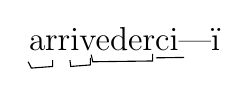
\begin{tikzpicture}[x=1cm,y=1cm]
\node[anchor=base west,inner sep=0pt] at (0,0) {\large arrivederc\unsure{i|ï}};
\draw (0,-.14)--(.04,-.22)--(.31,-.2)--(.31,-.12);
\draw (.53,-.12)--(.54,-.2)--(.79,-.18)--(.79,-.09);
\draw (.80,-.05)--(.82,-.14)--(1.58,-.13)--(1.58,-.04);
\draw (1.62,-.09)--(1.98,-.085);
\end{tikzpicture}}

\[
\left[\begin{array}{l}
\text{buon giorno}\\
\text{b\deleted{\unsure{uo}}uona se\deleted{\unsure{g}}ra}\\
\text{buona notte}\\
\text{per favore}\\
\text{mangare}\\
\text{col\deleted{\unsure{l}}\unsure{l}a\deleted{\unsure{g}}\unsure{z}ione}
\end{array}\right.
\]

% Street labels written sideways and slanted, following the road.
\figure{\begin{tikzpicture}[x=.010cm,y=-.010cm,line cap=round,line join=round]
\node[rotate=84,anchor=west,inner sep=0pt] at (96,224) {Corso Italia};
\draw (111,98)--(121,96)--(122,145)--(110,147)--cycle;
\node[rotate=40,anchor=west,inner sep=0pt] at (124,113) {\unsure{Pizzario|Pizzaria}};
\draw (112,232)--(116,305) (2,315)--(107,309);
\draw (167,225)--(177,304) (188,302) .. controls (242,298) and (311,305) .. (382,302);
\draw (18,377) .. controls (51,372) and (73,379) .. (99,374);
\draw (116,386)--(124,579)--(128,583) (10,575)--(110,572);
\draw (177,365)--(174,574) .. controls (235,576) and (306,570) .. (356,581);
\draw (182,356) .. controls (223,349) and (263,368) .. (331,357);
\draw (2,636)--(96,630) (116,633)--(121,824) (125,634)--(119,676)--(136,735);
\draw[->] (185,633) .. controls (192,703) and (185,747) .. (181,802);
\draw (152,633)--(361,631)--(366,668)--(444,663)--(450,634)--(386,626);
\node at (416,645) {$\unsure{v|\vee}$};
\draw (220,698) .. controls (237,717) and (224,814) .. (211,831)--(193,826)
 .. controls (255,852) and (221,999) .. (202,994)--(192,992)
 .. controls (232,1020) and (228,1160) .. (210,1154);
\draw (587,758)--(439,771)--(444,887)--(572,887);
\draw (601,765)--(606,864)--(597,877) (604,860)--(609,889)--(597,890) (590,894)--(584,894);
\end{tikzpicture}}
% archive sheet number: 5

\scanpage{7}
\[
A_n=A/(F^{n+1},V^{n+1})
\]
\[
I_n=A_n\quad\text{regardé comme \uline{bimodule} sur }A
\]
\[
\underline{I=\underset{n}{\varinjlim} I_n}\qquad I_n\overset p{\unsure{\mathord{-}|\longrightarrow}}I_{n+1}
\]
\[
D:M\leadsto\operatorname{Hom}(M,I)\unsure{'|\mathord{.}}\quad\text{foncteur dualisant}
\]

\uline{Attention}, à priori un module à g. est transformé en module à droite, et vice versa. Mais on peut utiliser l'involution $s$ de $A$, échangeant $F$ et $V$, pour passer de l'un à l'autre

\deleted{$D(M)$}\quad $A_n$ est fini sur $W_n$

Un autre foncteur dualisant est obtenu en faisant (si $M$ tué par $F^n,V^n$)
\[
D':M\leadsto\operatorname{Hom}_{W_n\text{-modules}}(M,W_n)
\]
et définissant sur $D'(M)$ la structure de $A$-module à droite par ``\unsure{transport.|transport|transpos.}''

\[
D'(\unsure{A_n|A|M})\unsure{\simeq|=}\operatorname{Hom}(A_n,W_n)\quad\text{structure de bimodule}
\]
\deleted{\unsure{Or|On}
\[
\operatorname{Hom}_{W_n}(M,W_n)=\operatorname{Hom}_{A_n}\bigl(M,\underbrace{\operatorname{Hom}_{W_n}(A_n,W_n)}_{\substack{\text{structure}\\\text{de bimodule}\\\text{naturelle}}}\bigr)
\]
Je dis qu'on a un \unsure{isom|isom.}
\[
I_n=A_n\simeq\operatorname{Hom}_{W_n}(A_n,W_n)
\]}
\deleted{$uF=u\circ F$}
% archive sheet number: 6

\scanpage{8}
\[
D'(M)=\operatorname{Hom}_{W_n}(M,W_n)\quad\text{module \uline{à droite} sur }A_n
\]
\[
\deleted{uF\ Fu\quad(uF)(x)=(u(F(x)))^{\pi^{-1}}}
\]
\[
\begin{aligned}
u\cdot F&=\pi^{-1}(u\circ F)&\quad\big| \quad u.F.V&=\pi\pi^{-1}u\circ F\circ V\\
u.V&=\pi(u\circ F)&\big|&=pu\\
u.\lambda&=u\circ\lambda&\big|\quad uVF&=pu\ \mathord{---}
\end{aligned}
\]
\[
D'(A_n)=\operatorname{Hom}_{W_n}((A_n)_g,W_n)\qquad\text{\uline{bimodule} sur }A_n
\]
\[
\begin{aligned}
u.F&=\pi^{-1}(u\circ F_g)\\
u.V&=\pi(u\circ V_g)\\
u.\lambda&=u\circ\underline{\lambda_g}&\quad u.\lambda&=\lambda.u=u\circ\lambda=\lambda\circ u\\
Fu&=u\circ F_d\\
\deleted{\unsure{F}}V\unsure{v|u}&\unsure{{:}|=}u\circ F_g\\
\lambda v&=u\circ\lambda_d
\end{aligned}
\]

\margin{\uline{attention} les deux structures \unsure{de|en} $W_n$ module sur $I'_n$ ne \unsure{st|sont} pas les \unsure{$\Rightarrow$|mêmes}}

\[
A_n\xrightarrow{\overset{?}{\sim}}\operatorname{Hom}_{\unsure{V_n|W_n}}((A_n)_g,W_n)
\qquad\text{\uline{isom de bimodules}}
\]
\[
\boxed{A_n\times A_n\longrightarrow W_n}
\]
\[
(x,y)\leadsto\langle x,y\rangle\qquad\text{\uline{biadditif}}
\]
\[
\begin{aligned}
\times\quad\langle\lambda x,y\rangle&=\lambda\langle x,y\rangle \qquad \lambda\in W_n\\
&\qquad\text{\unsure{donne} } A_n\xrightarrow{\text{\unsure{add.|à dr.}}}\operatorname{Hom}_{W_n}(\unsure{A_g|A_{ng}|(A_n)_g},W_n)
\end{aligned}
\]
\[
\left.\begin{aligned}
\times\quad\langle x,y\lambda\rangle&=\langle\lambda x,y\rangle\qquad\lambda\in W_n\\
\langle x,yF\rangle&=\pi^{-1}\langle Fx,y\rangle\\
\langle x,yV\rangle&=\pi\langle Vx,y\rangle
\end{aligned}\right\}\quad\text{assure }\swarrow\ \text{est }A_n\text{-lin. à \uline{droite}.}
\]
\[
\left.\begin{aligned}
&\left\{\begin{aligned}
\times\quad\langle x,\lambda y\rangle&=\langle x\lambda,y\rangle\\
\times\quad\langle x,Fy\rangle&=\langle xF,y\rangle
\end{aligned}\right.\\
&\times\quad\langle x,Vy\rangle=\langle xV,y\rangle
\end{aligned}\right\}\quad\text{assure }\swarrow\ \text{est }A_n\text{-lin.}
\]
\[
\deleted{\unsure{F^i F^j|F}}\qquad\deleted{\langle x,y\rangle}\qquad
\deleted{\langle x,y\rangle=\langle1,xy\rangle}\quad
\begin{aligned}\langle x,y\rangle&=\langle1,xy\rangle\\&=\langle xy,1\rangle\end{aligned}
\]

\noindent\begin{tabular}{|p{.92\linewidth}|}\hline
\diagram{\begin{tikzcd}[ampersand replacement=\&,column sep=small,row sep=small]
A_n\&[-1em]\otimes_{A_n}\&[-1em]A_n\arrow[r]\&\deleted{\unsure{A_n}}W_n\& W_n\text{-bilinéaire}\\
W_n\arrow[u,dash,sloped]\&\&W_n\arrow[u,dash]\&\deleted{\unsure{W_n\quad W_n}}\arrow[u,dash]\&
\end{tikzcd}}
\[
\begin{aligned}
\deleted{\pi\langle x,yF\rangle}&\quad\langle Fx,y\rangle=\pi\langle x,yF\rangle\\[-2pt]
\swarrow&\quad\langle x,yV\rangle=\pi\langle Vx,y\rangle
\end{aligned}
\]
\tabularnewline
\end{tabular}
% archive sheet number: 7

\scanpage{9}
% The writing is upside down relative to the archive foliation. Four long pen strokes cancel the sheet.
\deleted{\uline{Question} Comment définir directement une connexion intégrable sur $\mathbb R^{*}f_{*}(\Omega^{\cdot}_{X/S})$ ??

\uline{Lemme} $X$ Topos, $K^{\cdot},L^{\cdot}$ complexes abéliens de $X$, $\unsure{\mathscr G|\mathscr U|\mathscr Y|\mathcal G}$ faisceau abélien de $X$,
\[
\mathscr G\xrightarrow{i}\underline{\operatorname{Hom}}^{\cdot}(K^{\cdot},L^{\cdot})^{-1}
=\prod_i\underline{\operatorname{Hom}}(K^i,L^{i-1})
\]
$P$ un $\mathscr G$-torseur, $P\xrightarrow{\theta}\unsure{Z|\mathbb Z}(\underline{\operatorname{Hom}}(K^{\cdot},L^{\cdot})^{(0)})$

\deleted{Alors on peut associer à $P$ un homomorphisme de $D(X)$, de degré $0$\quad $K^{\cdot}\longrightarrow$}

un homomorphisme compatible avec les opérations de $\underline{\operatorname{Hom}}(K^{\cdot},L^{\cdot})^{-1}$
\[
\theta(g.p)=\theta(p)+\underbrace{\bigl(d\circ i(g)+i(g)\circ d\bigr)}_{\delta(i(g))}
\]
Alors on peut trouver un hom \uline{dans} $D(X)$
\[
\varphi=\varphi(\inserted{K,L,}\mathscr G,P,i,\deleted{\unsure{\varphi}}\theta):K^{\cdot}\longrightarrow L^{\cdot}
\]
tel que :

1\textsuperscript{o}) $\varphi$ est fonctoriel en $L^{\cdot}$ \inserted{\deleted{complexe} variable dans $C^{+}(X)$} (en un sens évident)

2\textsuperscript{o}) $\varphi$ est \deleted{fonctoriel} le \unsure{même} si on remplace \deleted{Si $\varphi$ peut être obtenu} $\mathscr G,P,i,\theta$ par $\mathscr G',P',i',\theta'$, avec $\mathscr G\xrightarrow{u}\mathscr G'$, $P\overset v{\unsure{\mathord{-}|\longrightarrow}}P'$, tels que $i=i'u$, $\theta=v\theta'$, $v$ \deleted{compatibles avec} un $u$-hom.

3\textsuperscript{o}) Si $P$ admet une section, alors}
% archive sheet number: 8

\scanpage{10}
\unsure{Caractères|Caractéres} des groupes de B.T. à réduction semi-stable virtuelle essentielle
% archive sheet number: 9

\scanpage{11}
\handwritten{\uline{Caractère} d'\uline{un groupe de} B.T \uline{sur un corps local}.}

Soit $V$ un anneau de val. discrète\inserted{\handwritten{\uline{à corps résiduel parfait}}}; pour ce qu'on va faire, on peut le supposer complet\handwritten{.} \deleted{à corps \uline{résiduel algébriquement clos} (\deleted{\unsure{peut être|peut-être|ce qui}} importe semble l'hypothèse corps résiduel parfait; on peut alors, au besoin, \inserted{\handwritten{(quitte à}} passer au complété de l'hensélisé strict).} On suppose que le corps résiduel $k$ de $V$ est de car. $p\handwritten{>}0$; le corps des fractions $K$ de $V$ est donc de car $p$ ou $0$ . On \deleted{si} s'intéresse aux\inserted{$p$-}groupes de Barsotti-Tate sur $K$, notés $M=(M(\handwritten{\nu}))_{\handwritten{\nu\geqslant}0}$ . On dit qu'un tel groupe \uline{satisfait à la condition de monodromie} s\deleted{i}'il admet une suite de composition par des groupes de B.T. , telle que les $\inserted{N=}\mathrm{Gr}^{i}(M)$ aient \uline{essentiellement bonne réduction}, i.e. qu'il existe pour chacun d'eux une extension finie \inserted{séparable} $K'$ de $K$ telle que \deleted{\unsure{sur $K$|sur $K'$}} $N_{K'}$ ait bonne réduction sur le normalisé $S'$ de $S$ dans $K'$. Alors $N_{K'}$ provient \deleted{d'un} donc, d'après le th. de Tate (démontré pour l'instant seulement dans le cas d'\inserted{in}égales caractéristiques), d'un \deleted{\unsure{schéma en}} groupe de B.T. $N$ sur $S'$ déterminé \uline{à isomorphisme unique près}. Par suite, si $K'$ est prise galoisienne de groupe $G$, $G$ opère sur \deleted{\unsure{ch|chaq}} $N$ de façon compatible avec son action sur $S'$. - Bien entendu, on peut prendre $K'$ indépendant de $i$ ; on dira, si $K'$ marche pour $M$ satisfaisant la condition de monodromie, que $K'$ est un \uline{corps de bonne réduction virtuelle} pour $M$.

Soit $K_{\mathrm{BT}}(K;K')$ le groupe ``de Grothendieck'' \deleted{\unsure{déf|dé}} défini\deleted{\unsure{s}} par les groupes de BT sur $K$ admettant $K'$ comme corps de bonne réduction virtuelle. Alors, si $K'/K$ est galoisienne de groupe de Galois $G$, on trouve un homomorphisme n\deleted{\unsure{q}}aturel
\[
K_{\mathrm{BT}}(K;K')\handwritten{\longrightarrow}K_{\mathrm{BT}}(S';G)\ ,\tag*{\handwritten{(1)}}
\]
où le deuxième membre est le groupe de Grothendieck des groupes de B.T. sur $S'$ avec opérations de $G$ (compatibles aux opérations de $G$ sur $S'$).

D'ailleurs, $S$ étant complet donc hensélien, $S'$ est local, de sorte que,
% archive sheet number: 10

\scanpage{12}
si $s'$ est son point fermé, on trouve aussi un homomorphisme de restrictio\unsure{n}
\[
K_{\mathrm{BT}}(S',G)\handwritten{\longrightarrow}K_{\mathrm{BT}}(s',G)\ ,\tag*{\handwritten{(2)}}
\]
en notant que $G$ opère sur $s'$ (de façon pas nécessairement fidèle). Or,$k'=k(s')$ étant supposé \deleted{complet}\inserted{parfait}, on a un foncteur \uline{covariant} naturel
\[
\mathrm{BT}(s')\deleted{\unsure{G)}}\handwritten{\unsure{\mathord{-}|\longrightarrow}}\mathrm{Modlib}(W(k'))\ ,\quad
\handwritten{\text{et \unsure{$=$|même} vers }\mathrm{Cris}(k')}
\]
et comme $G$ opère sur $k'$, donc sur $W(k')$, \deleted{\unsure{on}}le foncteur précédent induit trivialement un foncteur
\[
\mathrm{BT}(s',G)\handwritten{\longrightarrow}\mathrm{Modli}\deleted{\unsure{g}}\mathrm b(W(k'),G),
\]
d'où par suite un homomorphisme
\[
K_{\mathrm{BT}}(s',G)\handwritten{\longrightarrow}K(\deleted{\unsure{Mo}}W(k'),G)\ .\tag*{\handwritten{(3)}}
\]
Composant (1),(2) et (3), on trouve un homomorphisme canonique
\[
K_{\mathrm{BT}}(K;K')\handwritten{\longrightarrow}K(W(k'),G)\ .\tag*{\handwritten{(4)}}
\]
Notons d'ailleurs que si $k$ est algébriquement clos, alors $G$ opère trivialement sur $k'$ donc sur $W(k')$, et on a alors
\[
K(W(k'),G)=R_{W(k')}(G)\ ;
\]
dans le cas général, il y a lieu d'introduire le groupe d'intertie $I\handwritten{\subset}G$, et on trouve un homomorphisme
\[
K(W(k'),G)\handwritten{\longrightarrow}K(W(\deleted{\unsure{j}}k'),I)^{\inserted{\handwritten{G\deleted{\unsure{/I}}}}}\handwritten{\simeq}R_{W(k')}(I)^{\handwritten{G/I}},
\]
\margin{\handwritten{\uline{NB} $G\deleted{\unsure{/I}}$ opère sur $R$ via ses opérations sur $I$ \uline{et} sur $W(k')$ par transport de structure}}
% slanted
\margin{\handwritten{On peut \unsure{distinguer|dire} suivant les \unsure{différentes pentes|différents points} \ldots.}}
d'où grâce à (4)
\[
K_{\mathrm{BT}}(K,K')\handwritten{\longrightarrow}R_{W(k')}(I)^{\handwritten{G\deleted{\unsure{/I}}}}
\handwritten{\big[}\handwritten{\longrightarrow}\mathrm{Cent}_{\handwritten{G}}(I,W(\handwritten{k}'))\ ,\tag*{\handwritten{(5)}}
\]
la dernière flèche étant la flèche trace. L'homomorphisme composé est appelé encore l'homomorphisme trace, l'image de $\mathrm{c}\handwritten{\ell}(M)$ dahs le dernier membre est appelé le \uline{caractère} du groupe de B.T. $M$ . On voit facilement que dans un sens évident, il ne dépend pas du choix du corps de bonne réduction virtuelle $K'$: la fonction caractère est alors envisagée comme fonction sur le \inserted{sous-}groupe d'inertie (infini) de $\mathrm{Gal}(\overline K/K)$.

Supposons que $M_{K'}$ soit \uline{constant}, de sorte que \deleted{\unsure{$M$ est un f $M$}} $T_p(M)$ est un faisceau $p$-adique localement constant (au sens technique
% archive sheet number: 11

\scanpage{13}
du terme). On voit alors facilement que le caractère de $M$ coïncide, sur les éléments de $I$ \uline{d'ordre premier à} $p$, avec le \uline{caractère modulaire} de la représentation de $I$ \deleted{définie} sur $\handwritten{\mathbb F}_p$ définie par $M(\handwritten{0})$\deleted{\handwritten{?}}. Comme, pour $K$ de caractéristique nulle, la donnée d'un groupe de BT sur $K$ revient à la donnée d'une représentation $p$-adique de $\mathrm{Gal}(\overline K/K)$ (dans un \deleted{\unsure{m|M}}Module libre de type fini sur $\underline{\mathrm Z}_p$), on peut se demander \deleted{si} s'il n'est pas vrai en tous cas que le caractère d'un $M$ (satisfaisant la condition de monodromie) est déterminé ainsi par la seule connaissance de $M(\mathrm o)={}_pM$ . Il n'en est rien, car si cette condition était vérifiée, on en déduirait facilement, en utilisant la théorie de Brauer des relèvements virtuels des représentations sur $\underline{\mathrm F}_p$ en représentations sur $\deleted{\unsure{F}}\underline{\mathrm Z}_p$ , que pour \uline{tout} $M_{\deleted{\unsure{K}}}$ satisfaisant la condition de monodromie, le caractère de $M$ coincide avec le caractère modulaire de $M(\mathrm o)$ sur les éléments d'ordre premier à $p$ de $I$. En particu\deleted{\unsure{l}}lier, si $M$ a bonne réduction, il s'ensuivrait que le caractère modulaire \inserted{de $M(\mathrm o)$} serait trivial dès que $M$ a bonne réduction. Or c'est déjà faux en prenant $M=\underline{\mathrm Z}_p(1)$, donc $M(\mathrm o\unsure{.})=\handwritten{\mu}_p$ , \deleted{\unsure{dan}} en se plaçant dans le cas où $K$ ne contient pas les racines $p$.èmes de $1$. Dans le cas où il l\deleted{\unsure{eur}}\handwritten{es} contient, au contraite, il n'y a pas d'ennuis pour les groupes de BT sur $K$ qui sur un $K'$ ont une bonne réduction qui est, soit de type constant (cf plus haut), soit de type multiplicatif, et il conviendrait alors d'examiner encore le cas où il est de type ind-unipotent sur la \deleted{fibre} point fermé.

% slanted
\margin{\handwritten{\uline{NB} Cela impliquerait que la fonction caractère est à valeurs dans $\mathbb Z_p\subset W(k')$, dès que $K$ contient les racines $p$-ièmes de $1$ [donc sur le sous-gpe correspondant de $I$, d'indice $\unsure{\mid p-1|p-1|(p-1)}$] \deleted{\unsure{C'est} \illegible{3}}}}

Cas test: soient $E_{\unsure{1|i}}$\deleted{\unsure{et|$E_2$}}\inserted{$(i=1,2)$} deux courbes elliptiques sur $K$,qui ont bonne réduction essentielle, $ {}_pE_1$ isomorphe à $ {}_pE_2$ , $K$ contient les racines $p$.èmes de $1$ , est-il vrai que les fonctions traces $\handwritten{\phi}_{E_1}$ et $\handwritten{\phi}_{E_2}$ sur le groupe d'inertie (qu'on peut, comme on sait, calculer aussi via les $T_{\handwritten{\ell}}$ pour $\handwritten{\ell}$ nombre premier \uline{quelconque}) sont égales \inserted{sur les éléments premiers à $p$} ? Le \deleted{\unsure{seul}} cas intéressant est celui où l'une au moins des deux courbes, après extension $K\handwritten{\longrightarrow}K'$, se réduit en une courbe à invariant de Hasse nul. Ou encore: si $A_{\handwritten{K}}$ sdhéma abélien sur $K$
% archive sheet number: 12

\scanpage{14}
(par exemple courbe ellipttque) est tel que $ {}_p A_K$ soit un groupe constant, alors est-il vrai que la trace $\handwritten{\phi}_E$ soit \deleted{nulle}\inserted{égale à $n=\dim A_K$} sur les \deleted{points}-éléments premiers à $p$ de $I$ ? (Seul le c\deleted{\unsure{q}}as de réduction non semi-stable de $A$ offre un problème; donc il faudrait ici trouver un exemple où le critère de réduction semi-stable de Raynaud est en défaut pour $\handwritten{\ell}=p$ !).

Dans le cas d'une courbe elliptique, et en car. rés. $\handwritten{\ne}2,\handwritten{3}$, prenant pour $K\handwritten{\unsure{'|(}}$ la plus petite extension sur laquelle on a réduction semi-stable, on trouve que $G$ est un sous-groupe de $\mathrm{Aut}(A_{s'})$, lequel \inserted{est cyclique} a\handwritten{(}$2,4$ ou $6$ élément\unsure{s}, donc est premier à $p$, et la question revient à celle de savoir si $\handwritten{\phi}_E$ est de valeur\deleted{\unsure{s}} constante égale à $2$, \deleted{si}\inserted{\handwritten{lorsque}} $ {}_p A$ est con\deleted{\unsure{s}}stant\deleted{\unsure{e}} \handwritten{(}et \deleted{\unsure{à}}si $K$ contient les racines $p$.èmes de l'unité\inserted{\handwritten{(?)}}; il suffit de regarder le cas où la courbe elliptique réduite, après extension $K\handwritten{\longrightarrow}K'$, est d'invariant de Hasse nul\handwritten{)}\deleted{\unsure{;}}.

% slanted
\margin{\handwritten{\uline{faux par} \uline{Tate}}}
% archive sheet number: 13

\scanpage{15}
\deleted{\unsure{Déformation|Déformations} des groupes de B.T. ordinaires}

\unsure{Determination|Détermination} des ``stratifications canoniques'' sur \deleted{\unsure{le}}les déformations.

\uline{L'isom. de nature globale}
\[
\boxed{\operatorname{\text{dét}} T_p(A)_{\text{\unsure{ét|et}}}\simeq\operatorname{\text{dét}} T_p(A^{*})_{\text{ét}}}
\]
% archive sheet number: 14

